After having introduced the concepts of smart homes and Zero Trust security to the reader, together with the other fundamental concepts for this work, the next chapter will primarily focus on the theoretical aspects of the thesis. The chapter itself is divided into three sections.\\
The opening section introduces the security concepts for both network architectures, together with their adoption of Zero Trust principles in smart homes. Subsequently, the reader is provided with a detailed overview of each of how these setups should operate and serve to enhance the security of a smart home setup.\\
The next section of the chapter is dedicated to the introduction of two categories of evaluation metrics for both architectures. With regard to the research questions, the first set of metrics, also known as the primary metrics, is centered around the security factors, derived from the aforementioned Zero Trust components in Chapter 2 and the CIA triad\cite{cia_article} with a view to evaluate the security of the smart home environments. The secondary set of metrics focuses on the subjective matter around the implementation and ease of use of the smart home architectures, introducing factors such as the duration of the start-up phase, platform support and complexity.\\
The final parts of this chapter are dedicated to the limitations and challenges of the aforementioned smart home environments. It criticizes their flaws from an implementation and security standpoint, pinpointing the particular challenges of implementing Zero Trust practices in smart homes.\\\\\\\\\\\\\\

\section{Proposed Architectures for Smart Home}
With the aim to provide a more robust security model for smart home networks and for its measures against implicit trust, the Zero Trust security model has been chosen to be integrated in said smart home architectures. Both the locally hosted and the cloud-hosted environments have a similar setup configuration, as they essentially depend on a host device (either an RPI or a VM) to run a home automation software as per the user's choice, e.g. Home Assistant, which serves to facilitate a default smart home environment.\\
After the initial setup, both environments have been conceptualized to first adopt their Zero Trust security configuration before integrating an IoT device in their SHS. The user then accesses the home automation instance by means of using the client page of the HA software through a Multi-factor Authentication (MFA) login mechanism with a TOTP token as a second factor or directly connect to the host device, establishing an SSH connection. While the former approach is the default way for users to interact with the SHS and the IoT devices within, the SSH tunnel is meant as a way to manage the host file system and extend configuration.\\
Following this, the user integrates their IoT devices into the smart home network, as the process for said integration deviates, depending on whether the environment is on-premise or in the cloud. Figure 3.1 depicts a concept diagram of the template for both smart home environments, as previously described.
\begin{figure}[H]
	\centering
	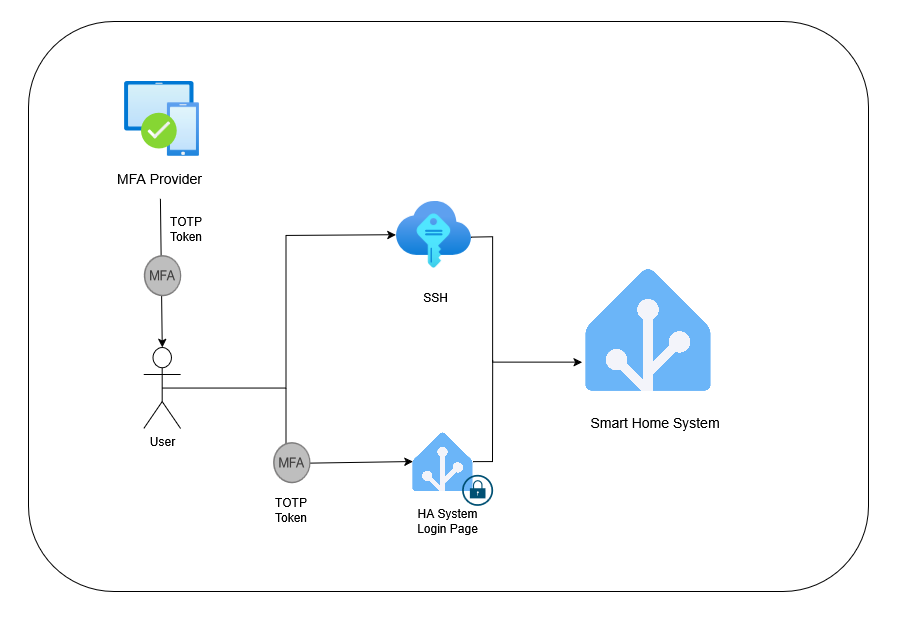
\includegraphics[width=0.8 \linewidth]{Images/shs-diagram.png}
	\caption{Smart Home Environment Concept Diagram}
	\label{fig:SHS_Arch}
\end{figure}

\subsection{On-Premise Architecture}
When considering the structure of an on-premise smart home architecture, it should be noted that its hardware comprises three synergizing main parts: the host device, gateway, and client device, as depicted in Figure 3.2.\\
\begin{figure}[H]
	\centering
	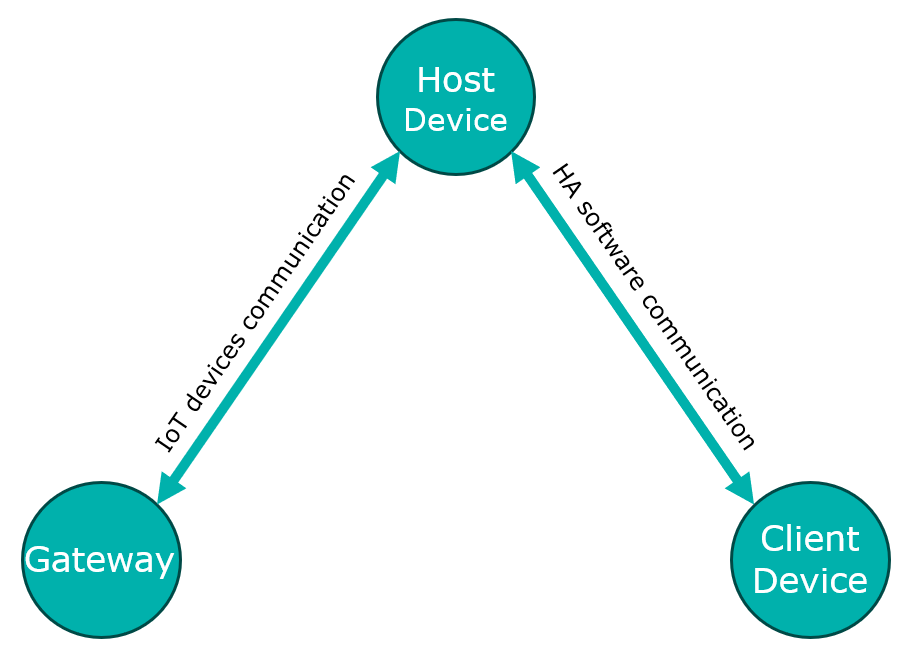
\includegraphics[width=0.6 \linewidth]{Images/smarthomearch.png}
	\caption{Main Components of a Smart Home Architecture}
	\label{fig:SHome_Comp}
\end{figure}

The host device is the one to operate the HA software, either as an OS in the case of Home Assistant\cite{home_assistant} or as a separate application and communicate with the user device. In the entire setup, it plays the role of the central hub, over which the communication between the IoT devices and the client device is established. Secondly, the gateway is responsible for the communication between the IoT devices and the host device, having no communication with the client device. Depending on the communication protocol over which the smart devices communicate, e.g. Zigbee, the gateway type may vary, as there is no universal gateway for all IoT devices. Together with the host device, they are the additional hardware required to get started with a SHS. As for the client device, it is usually a smartphone or a laptop, which connects to the personal area network at home. It allows the user to connect to the HA software instance running on the host device and either initiate actions with the IoT devices, e.g. adjust the colour temperature of a smart light bulb, or access information from their sensors, for instance room temperature from a temperature sensor.\\
Collectively, these three components create the basic smart home architecture, which, when integrated into the home network, provide the necessary environment for IoT devices to connect to. Integrating the IoT devices is usually done via a pairing process, depending on the protocol. The general principle is that a smart device will broadcast its presence and characteristics over the communication protocol (e.g. Zigbee) in the proximity before being paired. The pairing process is then initiated by the host device by sending a broadcast over the required gateway that it is available to pair. Once it picks up the IoT device's broadcast in a close radius, the process is then finished with both the IoT and the host device being successfully paired. Some IoT devices require the entering of a unique identifier pairing code for cases where there are several instances of the same device, as described in \cite{ha_homekit_bridge}.

\subsubsection{On-Premise Concept}
With regard to the concept of a Zero Trust architecture hosted locally, it has to be said that when conceptualizing the architecture, not all implementations of implicit trust principles in the network should be omitted. Instead, a more stable and user-friendly approach would be to combine the best aspects of both the Zero Trust and perimeter-based security principles for easier integration into the home network. Considering this, the core features of this architecture can be defined, as follows:

\begin{itemize}
\item Multi-Factor Authentication\\
  Multi-Factor Authentication is the authentication method of providing 2 or more credential types for user authentication. The credential types are based on information only the user should know(e.g. a password), own(e.g. a confirmation of identity over a client device) or identify as(e.g. fingerprints). Being one of the key principles of Zero Trust, the continuous authentication can be implemented using MFA for all users of the HA software. With this approach, each time a user logs in to manage or check the status of an IoT device over the HA software, e.g. Home Assistant, their identity can be proven with an additional factor, without implicitly trusting the entity logging in with a correct password as the user. When considering what additional factors are to be added to the authentication process, a more straightforward combination is the tuple of a password and a TOTP through an MFA service provider, as shown in Chapter 4.
  
\item Least Privilege Access\\
  With Least Privilege Access, users and entities are granted the minimum level of access within a network to complete their tasks. Implementing it for users in the HA platform can reduce the impact an attacker's breach has on the smart home network by reducing the amount of information and control a user profile has for certain IoT devices. In this context, the implementation of said feature depends on the features of the HA platform.
  
\item Firewall Rules over a Remote Tunnel\\
  A remote tunnel is in its entirety a proxy name for the default address of the HA instance in the user local area network (LAN). While the access to the HA platform instance should mostly be achieved from the LAN in an on-premise architecture, integrating a remote tunnel over the encrypted HTTPS protocol and enforcing a set of firewall rules provides a trade-off for being able to access the HA software. Depending on its capabilities, these firewall rules can range from restricting the access to the remote tunnel to a certain range of IP addresses to implementing an IP address ban on users after a number of login attempts has been exceeded. To achieve this in a local environment, it is crucial that the HA platform supports the integration of additional applications, for instance through add-ons, making it that more straightforward for users to configure.
  
\item Tunnel Analytics \& Alarms\\
  Moreover, the implementation of a remote tunnel should allow users to track general and web traffic analytics, such as number of requests sent, unique visitors over IP, etc. How this is beneficial for the security of the network is not that it directly prevents, but tracks, patterns of malicious activity. Combined with a set of alarm rules which either further restrict the access to the remote connection or simply shut off the connection, should a malicious attack pattern becomes more prominent over the tunnel, this makes the tunnel an important asset for the security of a local smart home network. 
\end{itemize}

\subsection{Cloud Architecture}
While the on-premise architecture requires several pieces of hardware as a base, setting up a smart home cloud architecture is more straightforward, as it requires just a client device with a stable enough internet connection. The hardware part which acts as a host device comprises a virtual machine provided by a cloud service provider, e.g. Amazon Web Services. However, a more complex aspect of this setup is the provisioning of the hardware and network resources for the VM as a host device.\\
Additionally, the establishing of a connection of a IoT device with the host device is not as easily done as when pairing in an on-premise architecture. For this purpose, either a virtual home gateway is needed, tailored to the specific needs of the cloud architecture or, as a broader approach, utilizing a proprietary gateway, which depends on the cloud service provider.

\subsubsection{Cloud Concept}
Regarding the Zero Trust cloud architecture in the cloud, the major conceptualization prerequisite is the same one followed by the on-premise solution -- it is by combining the best aspects of the Zero Trust and perimeter-based security, that this smart home cloud concept can be considered constructive. As for the core features of this architecture, they remain largely the same, but are implemented differently from the on-premise architecture:

\begin{itemize}
    \item \textit{Multi-Factor Authentication}\\
    In the case of using a cloud service provider (CSP) for hosting the smart home environment, it is possible to implement MFA on several instances. For starters, MFA can first be a component of logging into the CSP account of the user. Moreover, MFA can also be applied in the same manner as in the on-premise architecture -- by requiring each user profile in the hosted HA software to be authenticated using a TOTP. This multi-layered utilization of MFA should be implemented to serve as a deterrent for unauthorized access to the user's profile.
    Additionally, the second factor for an MFA process, e.g. the TOTP, should not be stored or delivered over third-party channels, only being accessible using an MFA provider service.
    
    \item \textit{Least Privilege Infrastructure Provision}\\
    When designing the cloud architecture for hosting a smart home, the principle of Least Privilege can be applied in the same way as it is in the local HA platform environment. Nevertheless, in the case of AWS as a CSP, the user is allowed to finetune the hardware specifications of the VM as provisioned infrastructure. Using an IaC tool like Terraform, it is possible to allocate just enough resources for the provisioned virtual machine to run effectively, according to the number of IoT devices and their function. Additionally, as the IaC concept was already introduced, it is possible to restrict the incoming and outgoing traffic both over specific ports, implementing a traffic filter of sort, and for certain IP address ranges only, by modifying the configuration scripts for the provisioned infrastructure.
\end{itemize}

\section{Evaluation Metrics}
In the process of working on both of the described architectures, there is an inherent need for performance indicator metrics through which to determine their utility and provide some insights into the following research questions:
\begin{itemize}
    \item How well is the Zero Trust paradigm integrated into a smart home environment?
    \item Should a Zero Trust smart home network be hosted locally or in the cloud?
\end{itemize}

For this purpose, the following group of important KPI measurements related to the research questions have been defined, as depicted in Table 3.1. The metrics themselves are divided into three categories: primary (also security) metrics and secondary metrics.\\
Starting with the security metrics, the first two represent the integrity and availability of devices, as part of the CIA triad \cite{cia_article}, since it is absolutely essential that sensor data over the smart home network is immutable and not serve as a way to sabotage the SHS. Moreover, the user should be able to fully access and modify their SHS, including but not limited to sensor data, configurations, automations, etc. 
The following two metrics relate to the ability of the smart home architecture to automatically update its system, and any services or applications currently operating on it, as well as provide users with the ability to create either partial or complete backups of the SHS configuration. The most important aspects of these two requirements are to be seamless and straightforward, regardless of the experience level of users, along with a well-documented setup process. In this context, the Home Assistant HA software introduced in Chapter 2 excels at fulfilling the aforementioned metric criteria \cite{ha_auto_update}, \cite{ha_auto_backups}, \cite{ha_backup_integration}. 
The last of the security metrics is derived from the set of ZT principles defined in Chapter 2. While not directly contributing to the security integrity of the environment, the ability of a SHS to monitor device activity and trigger alarms for certain anomaly patterns, e.g. temperature sensor data fluctuating too rapidly or being outside the typical range, contributes to creating a privacy-conscious environment for users.\\
With respect to the last three metrics in the table, they are designated as secondary metrics and thus cannot be measured due to them being subjective. The reasons for that are, these measurements depend on a variety of subjective factors, mainly user experience and the functionality of both the smart home and hosting platforms, which are nonetheless just as influential for the adoption of the Zero Trust paradigm in smart homes.\\
The first one, measuring the duration until a simple ZT smart home instance is operational, is significant in the context of users being able to readily scale their smart home architectures and is most heavily influenced by the level of experience the user has. The latter two relate to the smart home (e.g. Home Assistant) and the hosting (e.g. Amazon Web Services) platforms utilized in creating the HA instance. Despite the fact that these services may offer a great amount of assistance for implementing ZT security, it should not be overlooked that an excess of functionality may cause confusion amongst users. Consequently, it is critical for smart home architectures in the context of Zero Trust to be balanced in terms of platform support and complexity.

\begin{table}[H]
    \centering
    \footnotesize
    \setlength{\tabcolsep}{6pt}
    \begin{tabularx}{\dimexpr\textwidth-6\columnsep\relax}{|c|c|X|}
        \hline
        Metric & Unit & Description \\
        \hline 
        Device Integrity & \% & The ratio of secure and functional devices without known vulnerabilities. \\
        \hline
        Device Availability & \% & The ratio of fully operational devices. \\
        \hline
        Automatic Updates & Yes/No & The ability for services to be automatically updates without user guidance. \\
        \hline
        Automatic Backups & Yes/No & The ability for services to provide an automatic backup of the user's configuration. \\
        \hline
        Device Alarms and Monitoring & Yes/No
        & The ability of the smart home system to monitor device and user activity and alarm users for anomalous behaviour. \\
        \hline
        Duration of start-up phase & nil & This metric refers to the time it takes to start from an empty original state to a simple smart home instance implementing ZT. \\
        \hline
        Platform Support & nil & This metric refers to the amount of mechanisms, tools, and tips for overall and ZT security principles the user has at their disposal. \\
        \hline
        Platform Complexity & nil & This metric refers to the amount of functionality and features the platforms offers, an overabundance of which may cause difficulties for the end user. \\
        \hline
    \end{tabularx}
    \caption{Metrics Overview Table}
\end{table}

\section{Limitations}
When considering the limitations of the introduced smart home architectures, it should be noted that the conceptualized security measures are primarily intended to be deployed in a consumer IoT environment and are therefore unfit for environments as part of the Industrial Internet of Things (IIoT) \cite{iiot_article}. This notion is in view of the fact that the security challenges as part of industrial environments are different to those in consumer ones on account of the longer lifetime of industrial-grade devices, the larger scale of IIoT device networks and their dynamic interconnection between field, controller devices and servers \cite{iiot_challenges}.\\
As most security approaches for consumer IoT place the emphasis on the security of individual devices and services within the IoT environment, the need to secure connections between devices and their automated tasks is not directly addressed. This is also true for the current iterations of both ZT smart home architectures submitted as part of this work. Whereas these architectures focus on user-centric security measures for these environments, e.g. MFA, Principle of Least Privilege, firewall-based remote access, etc., they do not take into consideration the specific IIoT demands for security to be customized to the resource constraints of devices. \cite{iiot_challenges}\\
Consequently, this section provides concise insights on the limitations and challenges for smart home implementations, established on the aforementioned on-premise and cloud ZT network architectures, which serve as a base for the implementation and findings assessment in Chapter 5 of this work.

\subsection{On-Premise Architecture}
\subsubsection{Plugins as a security risk}
While the on-premise architecture can definitely benefit from the adoption of security-related plugins, it is entirely possible that the plugins themselves contain zero-day vulnerabilities, which can compromise the smart home network. In the context of Home Assistant, these so-called add-ons are primarily open-source software without any security guarantees and could pose a security risk for the smart home network. 

\subsubsection{Instability of services}
The services used to enforce security measures through plugins can also be slow or unstable due to resource constraints. As the local smart home environment is conceptualized to operate on an SBC, the connection to the remote tunnel may prove unstable or even inactive, prompting a restart of the system. If such events occur one too many times, the boundaries between security and user-friendliness of the on-premise architecture become ambiguous.

\subsection{Cloud Architecture}
\subsubsection{IoT Device connection}
As connecting an IoT device with the HA platform in the cloud is not that straightforward of a process, requiring either a virtual or a proprietary gateway, this introduces additional difficulty for new users. From a security perspective, this also expands the attack surface of the network in comparison with the on-premise architecture.

\subsubsection{Virtual Machine Setup}
When first setting up the virtual machine in the cloud, a starter script is required to run for it to host the HA software, provided it is operated as a container. If a similar way to the local architecture is chosen to set up the environment through an OS for home automation, this prompts the creation of a specific virtual machine image with the desired configuration, further complicating the cloud environment setup process.